\documentclass[a4paper, 12pt]{article}

\usepackage{amsfonts, amsmath, amssymb}
\usepackage[english]{babel}
\usepackage[style=alphabetic]{biblatex}
\addbibresource{bibliography.bib}
\usepackage{csquotes}
\usepackage[a4paper,left=1.4cm,right=1.4cm,top=2cm,bottom=2cm]{geometry}
\usepackage[colorlinks=true, allcolors=blue]{hyperref}
\usepackage{mathtools}
\usepackage{nicematrix}
\usepackage{tikz}
\usepackage[dvipsnames]{xcolor}

\setlength{\parindent}{0pt}

\title{Shortest Path Problem in Affine Subspaces}
\author{}
\date{\vspace{-1cm}\today}

\begin{document}
\maketitle

\begin{abstract}
    In this short document, we describe the problem of finding the shortest path between a source $s$ and a target $t$, both in $\mathbb{R}^n$, while staying on affine subspaces $\{x \in \mathbb{R}^n \vert A_i x + b_i = 0\}, i = 1, \dots, m$. In the~\hyperref[sec:statement]{first section}, we introduce the problem and the notations used. Then, in section~\ref{sec:modelization}, we modelize it as a Shortest Path Problem (SPP) in a Graph of Convex Sets (GCS). We will explore two approaches for this. In the~\hyperref[sec:experiments]{last section}, we will discuss the pros and cons of both methods, based on expiments in Julia.
\end{abstract}

\section{Problem statement}\label{sec:statement}
Let $s, t \in \mathbb{R}^n$ denote a source and a target respectively. Given a set of parameters \[{\left\{(A_i, b_i)\right\}}_{i=1}^{m} \subset \mathbb{R}^{d \times n} \times \mathbb{R}^d,\] we would like to find a path $q : [0,T] \mapsto \mathbb{R}^n$, with $q(0) = s$ and $q(T) = t$, such that, \[\forall \tau \in [0,T], \exists i \in \{1, \dots, m\} : A_i q(\tau) + b_i = 0.\] We will assume throughout this work that $s$ and $t$ belong to at least one of those affine subspaces. If it is not the case, trivially, such a path does not exist. The value of $T$ may be interpreted as the time at which we reach the target, or the length of the path between the source and the target.\\
In addition to this, we associate to each affine subspace a cost $\beta_i \in \mathbb{R}_{\geq 0}, i = 1, \dots, m$, representing the price to pay for staying on the corresponding affine subspace.

An example of such a problem in two dimensions is given in figure~\ref{fig:SPP-problem}.

\begin{figure}[!htb]
    \centering
    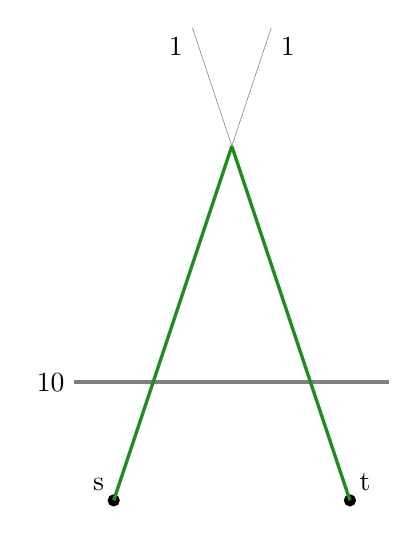
\begin{tikzpicture}
        \draw[gray, ultra thick] (-2,0) -- (2,0);
        \node[anchor=east] at (-2,0) {10};
        \draw[gray, very thin] (-0.5,4.5) -- (1.5,-1.5);
        \node[anchor=north east] at (-0.5,4.5) {1};
        \draw[gray, very thin] (-1.5,-1.5) -- (0.5,4.5);
        \node[anchor=north west] at (0.5,4.5) {1};

        \filldraw[black] (-1.5,-1.5) circle (2pt)
        node[anchor=south east] {s};
        \filldraw[black] (1.5,-1.5) circle (2pt)
        node[anchor=south west] {t};

        \draw[ForestGreen, very thick] (-1.5,-1.5) -- (0,3);
        \draw[ForestGreen, very thick] (0,3) -- (1.5,-1.5);
    \end{tikzpicture}
    \caption{Example of an SPP in which the path has to stay on given affine subspaces. In this example, we have three affine subspaces, of cost $10$, $1$ and $1$ respectively. The shortest path between the source $s$ and the target $t$ is represented in green. Notice that the high cost of the horizontal line prevents of using it.}\label{fig:SPP-problem}
\end{figure}

\section{Modelization}\label{sec:modelization}
In this section, we modelize mathematically the problem as a Shortest Path Problem (SPP) in a Graph of Convex Sets (GCS). GCS is a framework used to modelize graphs whose vertices are convex sets. It has been introduced in Tobia Marcucci's thesis~\cite{Tobia}, and may be used for several applications, like robot motion planning.\\
We see at least two ways to tackle this problem. The first one is by considering a graph in which the vertices are given by the intersection of the affine subspaces, and the edges by the subspaces themselves. This first approach is expended in subsection~\ref{subsec:vertices}. An alternative, based on what is done in~\cite[Chapter~11]{Tobia} for motion planning, is to consider the subspaces as the vertices, binding two subspaces by an edge if they have an intersection. This is detailed in subsection~\ref{subsec:edges}.

\subsection{Intersections as vertices}\label{subsec:vertices}
The first possibility is to construct a graph whose vertices are the intersections between affine subspaces, and whose edges are the affine subspaces, i.e., there is an edge between two vertices if they belong to a same affine subspace. We add to this graph two vertices, one for the source $s$ and one for the target $t$, associated with a singleton corresponding to there coordinates. For example, the GCS corresponding to the problem of figure~\ref{fig:SPP-problem} is drawn in figure~\ref{fig:vertices}. There are five vertices, corresponding to the three intersections, the source and the target.

\begin{figure}[!htb]
    \centering
    \begin{tikzpicture}[node distance={3cm}]
        \node[draw, circle] (1) {$\{(0,3)\}$};
        \node[draw, circle] (2) [below left of=1] {$\{(-1,0)\}$};
        \node[draw, circle] (3) [below right of=1] {$\{(1,0)\}$};
        \node[draw, circle] (4) [below left of=2] {$s$};
        \node[draw, circle] (5) [below right of=3] {$t$};

        \draw (1) to (2);
        \draw (1) to (3);
        \draw (1) to [out=180, in=135, looseness=1] (4);
        \draw (1) to [out=0, in=45, looseness=1] (5);
        \draw (2) to (3);
        \draw (2) to (4);
        \draw (3) to (5);
    \end{tikzpicture}
    \caption{GCS corresponding to the problem presented in figure~\ref{fig:SPP-problem}, with the intersections as vertices. The coordinates of the intersection points are there only for an illustration purpose, and were chosen randomly.}\label{fig:vertices}
\end{figure}

Let $v$ and $w$ be two nodes of the graph, associated with the convex regions $\mathcal{X}_v$ and $\mathcal{X}_w$ respectively, and linked by an edge $e$. The cost function on the edges is defined as
\begin{equation}\label{eq:f_e}
    f_e(\mathbf{x}_v, \mathbf{x}_w) = \beta_e {\lVert \mathbf{x}_v - \mathbf{x}_w \rVert}_2,
\end{equation}
where $\beta_e$ is the cost of the affine subspace linking the convex sets $\mathcal{X}_v$ and $\mathcal{X}_w$. There is no cost function on the vertices.

Since there are no costs on the vertices and the costs on the edges are nonnegative, we may use the formulation (9.5) from~\cite{Tobia}\footnote{Notice that we do not need the constraint (9.5f) as there is no constraint on the edges for this problem}. For convenience, we rewrite the model in~(\ref{eq:vertices}).

\begin{subequations}\label{eq:vertices}
    \begin{align}
    \text{minimize}\quad   & \sum_{e = [v,w] \in \mathcal{E}} \tilde{f}_e (\mathbf{z}_v^e, \mathbf{z}_w^e, y_e)\label{eq:vertices-a}\\
    \text{subject to}\quad & y_e \in \{0, 1\} & \forall e \in \mathcal{E}\label{eq:vertices-b}\\
                           & \sum_{e \in \mathcal{I}_v^{in}} y_e + \delta_{sv} = \sum_{e \in \mathcal{I}_v^{out}} y_e + \delta_{tv} \leq 1 & \forall v \in \mathcal{V}\label{eq:vertices-c}\\
                           & \sum_{e \in \mathcal{I}_v^{in}} \mathbf{z}_v^e = \sum_{e \in \mathcal{I}_v^{out}} \mathbf{z}_v^e & \forall v \in \mathcal{V} \setminus \{s, t\}\label{eq:vertices-d}\\
                           & (\mathbf{z}_v^e, y_e) \in \tilde{\mathcal{X}}_v & \forall v \in \mathcal{V}, e \in \mathcal{I}_v.\label{eq:vertices-e}
    \end{align}
\end{subequations}

Let us explicit the terms, emphasing their signification in this problem. The set $\mathcal{V}$ (resp. $\mathcal{E}$) contains the vertices (resp.~the edges) of the graph. To each vertex $v \in \mathcal{V}$, we associate a convex set $\mathcal{X}_v$, corresponding to the intersection of the two affine subspaces represented by this vertex. Let $(A_i, b_i)$ and $(A_j, b_j)$, $i \neq j \in \{1, \dots, m\}$ be the parameters of those subspaces. Then, $\mathcal{X}_v$ can be described explicitly by \[\mathcal{X}_v \coloneq \left\{x \left\lvert \begin{bmatrix} A_i \\ A_j \end{bmatrix} x + \begin{bmatrix} b_i \\ b_j \end{bmatrix} = 0 \right.\right\}.\] The set $\mathcal{I}_v$, $v \in \mathcal{V}$, contains all the edges incident to the vertex $v$.

We distinguish three different kind of variables:
\begin{itemize}
    \item $\mathbf{x}_v \in \mathbb{R}^n$ for all $v \in \mathcal{V}$, which are continuous random variables corresponding to the position of a point in the convex set of node $v$. These variables are constrained in the sets $\mathcal{X}_v$ if the shortest path goes through node $v$, which is hidden in the constraint~(\ref{eq:vertices-e});
    \item $y_e \in \{0,1\}$ for all $e \in \mathcal{E}$, which are binary variables, corresponding to the choice of taking the edge $e$ or not in the path;
    \item $\mathbf{z}_v^e \in \mathbb{R}^n$ for all $e \in \mathcal{I}_v$, for all $v \in \mathcal{V}$, which are auxiliary variables corresponding to the product of the two previous variables.
\end{itemize}
Notice that the variables $\mathbf{x}_v$ do not appear in model~(\ref{eq:vertices}), and the only decision variables that need to be given to the solver are $y_e$ and $\mathbf{z}_v^e$. We may then recover the values of the variables $\mathbf{x}_v$ at the vertices of the path as the value of $\mathbf{z}_v^e$ for an incident edge in the path (i.e., for which $y_e = 1$).

The objective function~(\ref{eq:vertices-a}) is the homogenization of the function $f_e$ defined in~(\ref{eq:f_e}):
\begin{equation}
    \tilde{f}_e(\mathbf{z}_v^e, \mathbf{z}_w^e, y_e) \quad = \quad \left\{ \begin{split} f_e(\mathbf{z}_v^e, \mathbf{z}_w^e) & \quad \text{if $y_e = 1$} \\ \infty & \quad \text{if $y_e = 0$}\end{split} \right. \quad = \quad \left\{ \begin{split} f_e(\mathbf{x}_v, \mathbf{x}_w) & \quad \text{if $y_e = 1$} \\ \infty & \quad \text{if $y_e = 0$}\end{split} \right. .
\end{equation}
The constraint~(\ref{eq:vertices-c}) can be seen as a flow equation, i.e., if a vertex is entered, then the path has to exit it. We have $\delta_{ij}$ is equal to one if and only if $i = j$. This allows to have a virtual unit entering the source node $s$ and a virtual unit exiting the target node $t$. These values can not be greater than $1$, to prevent the path of going several times through the same vertex. Finally, the constraint~(\ref{eq:vertices-d}) is a valid equality generated from constraint~(\ref{eq:vertices-c}), as described in~\cite[Remark 5.3]{Tobia}, and represents the continuity of the path.

\subsection{Intersections as edges\protect\footnote{Largely inspired from~\cite[Chapter 11.2]{Tobia}}}\label{subsec:edges}
The second option is to consider the intersections of affine subspaces as the edges, and taking for vertices the affine subspaces themselves, plus the source and the target. The source and target are linked by an edge to the subspace (potentially several) they are contained in. The corresponding GCS of the problem of figure~\ref{fig:SPP-problem} is drawn in figure~\ref{fig:edges}.

\begin{figure}[!htb]
    \centering
    \begin{tikzpicture}[node distance={3cm}]
        \node[draw, circle] (1) {$s$};
        \node[draw, circle] (2) [right of=1] {$A_1 x + b_1 = 0$};
        \node[draw, circle] (3) [right of=2] {$A_2 x + b_2 = 0$};
        \node[draw, circle] (4) [above of=3] {$A_3 x + b_3 = 0$};
        \node[draw, circle] (5) [above of=4] {$t$};

        \draw (1) to (2);
        \draw (2) to (3);
        \draw (2) to (4);
        \draw (3) to (4);
        \draw (4) to (5);
    \end{tikzpicture}
    \caption{GCS corresponding to the problem presented in figure~\ref{fig:SPP-problem}, with the intersections of subspaces as edges.}\label{fig:edges}
\end{figure}

Let $\mathcal{V}$ (resp. $\mathcal{E}$) be the set of vertices (resp. edges). For each affine subspace, we define the convex region \[\mathcal{C}_i \coloneq \{x \in \mathbb{R}^n \mid A_i x + b_i = 0\}, \qquad i = 1, \dots, m.\]
To each vertex $j \in \mathcal{V}\setminus\{s, t\}$, we associate the convex constraint set $\mathcal{X}_j \coloneq \mathcal{C}_j \times \mathcal{C}_j$. Therefore, the points inside those sets can be seen as pairs of two points in the affine subspace: the starting point and the ending point. Mathematically, $\mathbf{x}_i \coloneq (\mathbf{q}_{i,0}, \mathbf{q}_{i,1})$, with $\mathbf{q}_{i,0}, \mathbf{q}_{i,1} \in \mathbb{R}^n$. We associate a cost function on those vertices, begin the euclidean distance between the two points, multiplied by the cost of the affine subspace: \[f_i(\mathbf{x}_i) = \beta_i {\lVert \mathbf{q}_{i,0} - \mathbf{q}_{i,1} \rVert}_2, \qquad i = 1, \dots, m\]
For all the edges between two such vertices, we have to ensure the continuity of the path by imposing $\mathbf{q}_{i,1} = \mathbf{q}_{j,0}$, where $i$ and $j$ are the vertices incident to the edge.

The source and the target are paired with the singletons corresponding to their coordinates. No cost function is associated with them. We impose that for all vertex $i \in \mathcal{V}$ incident to the source (resp. target), $\mathbf{q}_{i,0}$ (resp. $\mathbf{q}_{i,1}$) is equal to the coordinates of $s$ (resp. $t$).

Finally, 

\section{Numerical experiments}\label{sec:experiments}

\printbibliography{}
\end{document}